\documentclass[12pt, oneside]{article}
\usepackage[letterpaper, margin=1in, headsep=0.5in]{geometry}
\usepackage[english]{babel}
\usepackage[utf8]{inputenc}
\usepackage{amsmath}
\usepackage{amsfonts}
\usepackage{amssymb}
\usepackage{tikz}
%\usetikzlibrary{quotes, angles}
\usepackage{graphicx}
%\usepackage{pgfplots}
%\pgfplotsset{width=10cm,compat=1.9}
%\usepgfplotslibrary{statistics}
%\usepackage{pgfplotstable}
%\usepackage{tkz-fct}
%\usepackage{venndiagram}

\usepackage{fancyhdr}
\pagestyle{fancy}
\fancyhf{}
\rhead{\thepage \\Name: \hspace{1.5in}.\\}
\lhead{BECA / Dr. Huson / Geometry 10.3\\* 15 October 2018}

\renewcommand{\headrulewidth}{0pt}

\begin{document}
\subsubsection*{Do Now: Graph equations}
  \vspace{0.5cm}

\begin{enumerate}
  \item   Given the equation: $y=x-2$.
  \begin{enumerate}
      \item Fill in the table of values on the left, from $-2$ to $3$.
      \item Mark points on the grid from the table
      \item Draw a straight line through the points
      \item Write down the slope and $y$-intercept. \vspace{3cm}

      \begin{center} %4 quadrant regents grid
      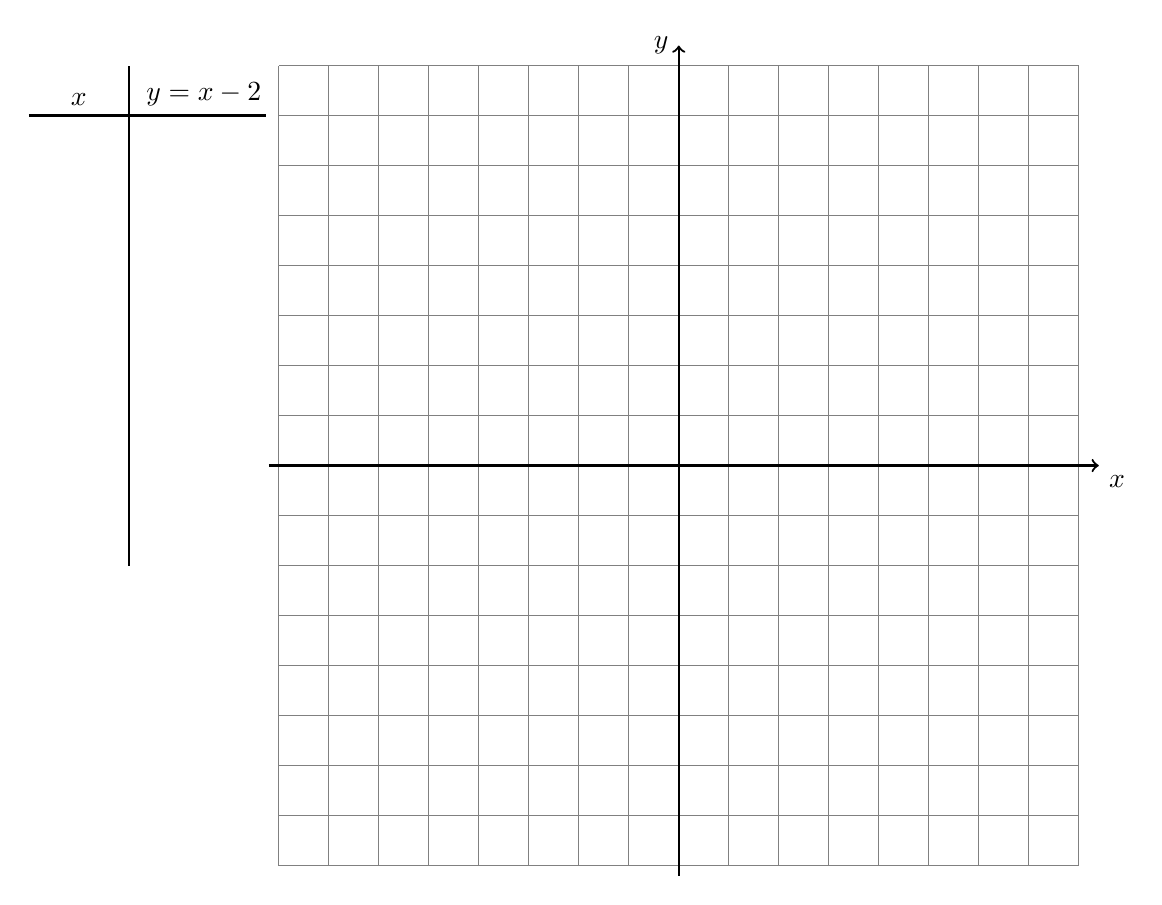
\begin{tikzpicture}[scale=.635]%[scale=0.635]
        \draw [thick, -] (-11, -2)--(-11,8);
        \draw [thick, -] (-13,7)--(-8.25,7);
        \node at (-12,7) [above] {$x$};
        \node at (-9.5,7) [above] {$y=x-2$};
        \draw [help lines] (-8,-8) grid (8,8);
        \draw [thick, ->] (-8.2,0) -- (8.4,0) node [below right] {$x$};
        \draw [thick, ->] (0,-8.2)--(0,8.4) node [left] {$y$};
      \end{tikzpicture}
      \end{center}

  \end{enumerate}


  \newpage
  \subsubsection*{Classwork: solve equations}
  Solve for the value of $x$.

  \item   $3x-8=x$ \vspace{3cm}
  \item   $12=3x-x$ \vspace{3cm}
  \item   $\frac{1}{2}(x+3)=2x$ \vspace{4cm}
  \item   $15=\frac{1}{2}x+2x$ \vspace{5cm}

  \item   What is the slope and $y$-intercept of $y=2x-4$?
    \vspace{2cm}
  \item   Convert to slope-intercept form: $4x+2y=8$ \vspace{3cm}

  \item Given $f(x)=-3x+5$. Simplify $f(2)$. \vspace{3cm}
  \item Given $\displaystyle g(x)=\frac{(15-4x)}{5}$. Simplify $g(0)$.  \vspace{3cm}

\newpage

\item Graph the function $f(x)=\frac{1}{2}x+4$.
\begin{enumerate}
    \item Write down the $y$-intercept.\\*[10pt]
    \item Write down the slope of $f(x)$.\\*[10pt]
    \item Label the intersection of $f(x)$ with the $x$-axis as the point $P$.
    \item Mark the point $Q (6, 2)$.
    \item A second line, $g(x)$, is parallel to $f(x)$ and passes through point $Q$. Plot $g(x)$ on the graph.
    \item What is the $y$-intercept of $g(x)$?
\end{enumerate}

\begin{center} %4 quadrant regents grid
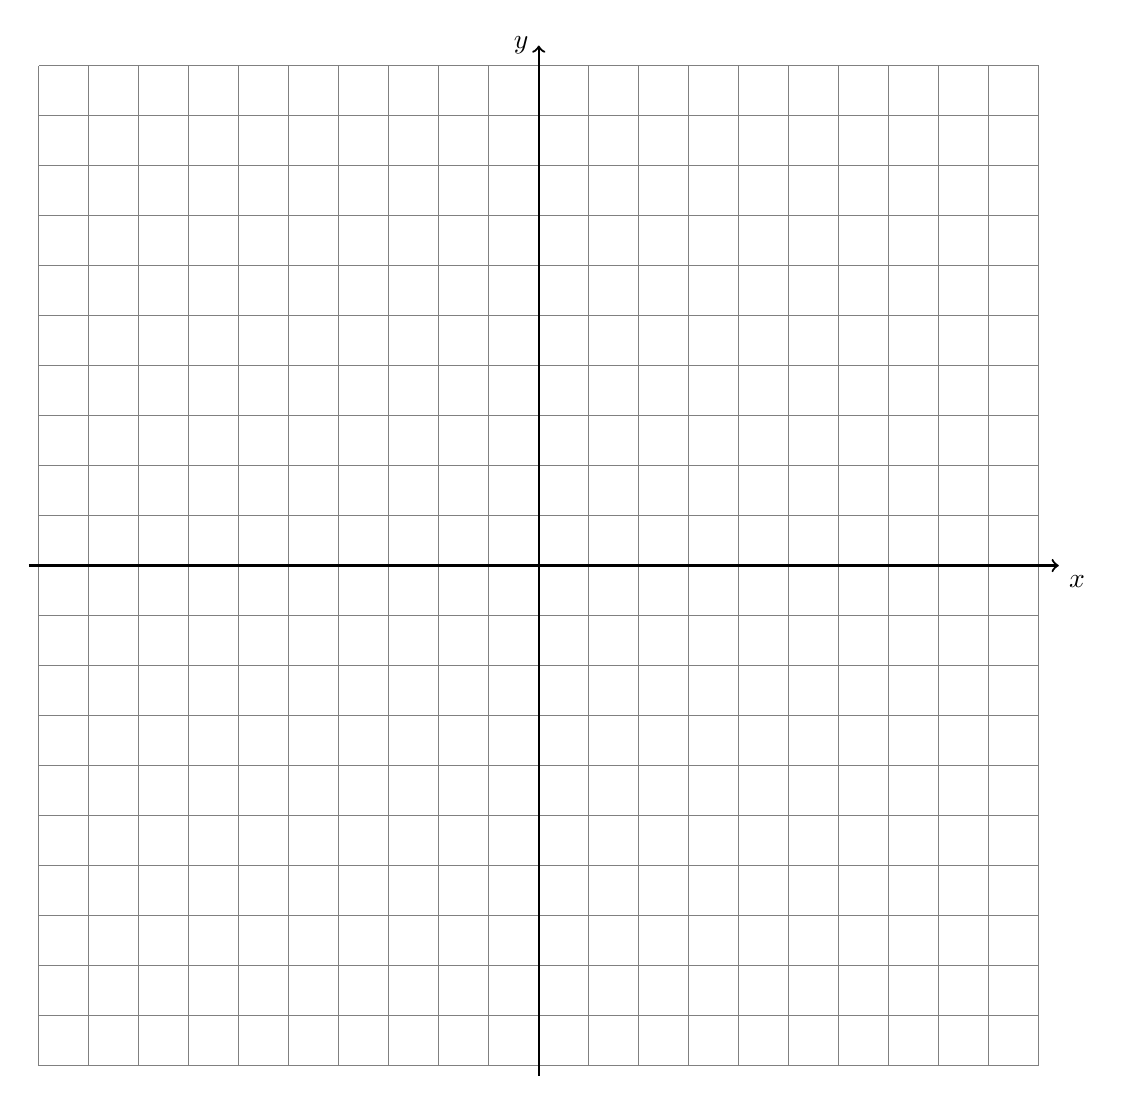
\begin{tikzpicture}[scale=.635]%[scale=0.635]
  \draw [help lines] (-10,-10) grid (10,10);
  \draw [thick, ->] (-10.2,0) -- (10.4,0) node [below right] {$x$};
  \draw [thick, ->] (0,-10.2)--(0,10.4) node [left] {$y$};
  %\draw[fill] (2,2) circle  [radius=0.05]
       %node[below left] (4, 2) {$A$};
\end{tikzpicture}
\end{center}

\newpage
\item
\begin{enumerate}
    \item Mark the point $P(3, -2)$ on the graph.
    \item The line $L_1$ has a $y$-intercept of 2 and passes through point $P$. Graph $L_1$.
    \item What is the slope of line $L_1$?\\*[20pt]
    \item What is the equation of line $L_1$?\\*[20pt]
    \item A second line, $L_2$ has the equation $x-y=-9$. Plot $L_2$ on the graph.
    \item What is the slope of $L_2$?\\*[30pt]
    \item Are the two lines $L_1$ and $L_2$ parallel, perpendicular, or neither?
  \begin{center} %4 quadrant regents grid
  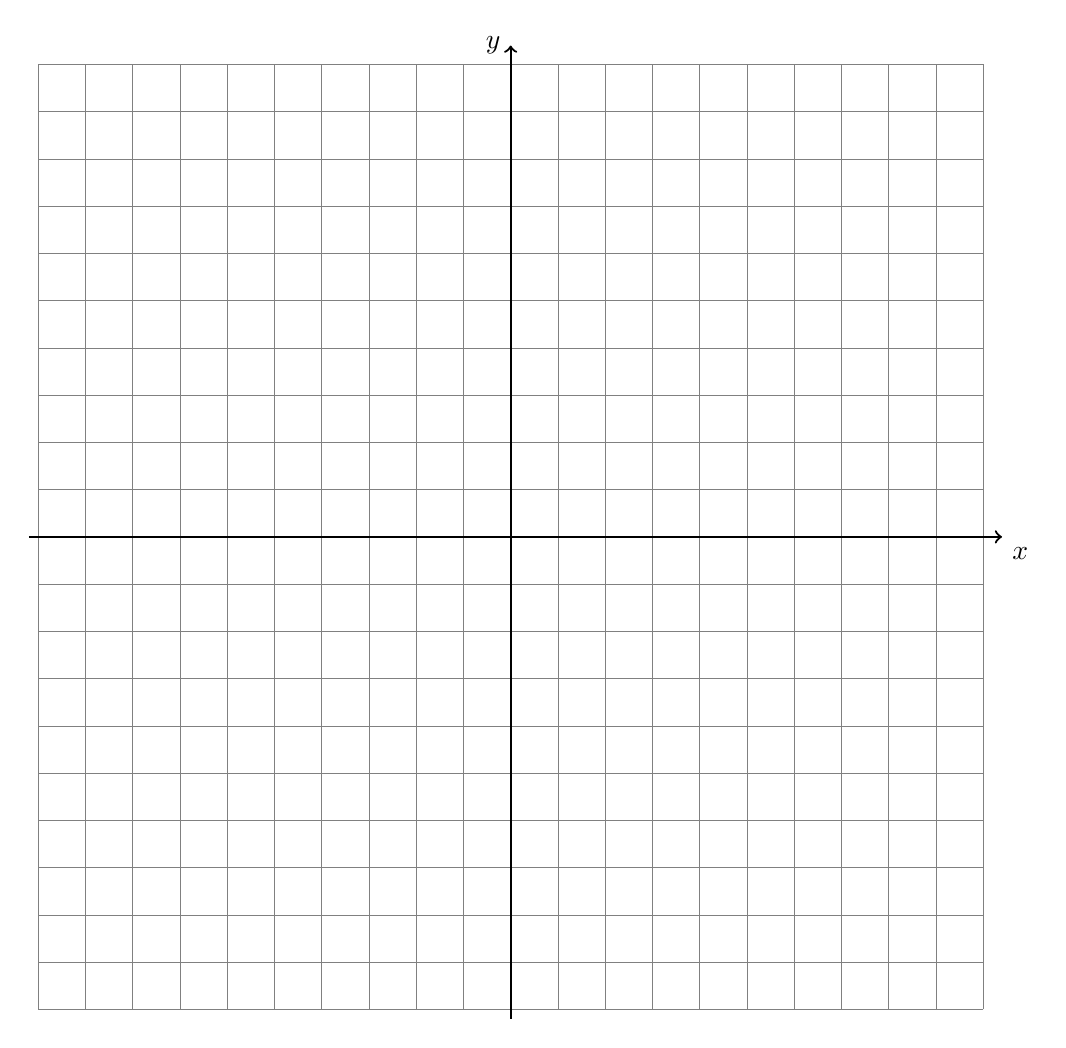
\begin{tikzpicture}[scale=.6]%[scale=0.635]
    \draw [help lines] (-10,-10) grid (10,10);
    \draw [thick, ->] (-10.2,0) -- (10.4,0) node [below right] {$x$};
    \draw [thick, ->] (0,-10.2)--(0,10.4) node [left] {$y$};
    %\draw[fill] (2,2) circle  [radius=0.05]
         %node[below left] (4, 2) {$A$};
  \end{tikzpicture}
  \end{center}

\end{enumerate}

\newpage
\subsection*{Point-slope form}

  \item What is the equation of the line with a slope of 2 passing through the point $(2,1)$? \vspace{4cm}
  \item What is the equation of a line parallel to $y=-x+4$ through the point $(3, 2)$? \vspace{4cm}
  \item What is the slope of a line perpendicular to the line $2x-4y=5$? \vspace{4cm}

\newpage
\subsection*{Model situations with linear functions}
  Use pencil and a straight edge to make a scatter plot and line of best fit.
  \item Label the axes as  $x$ and $y$. Mark at least some values (for example, 5, 10, 15, and 20).
  \begin{enumerate}
      \item Plot the values of $x$ and $y$ shown in the table.\\[5pt]
  	\begin{tabular}{|l|c|c|c|c|c|c|c|c|c|}
  	\hline
  	$x$ & 1 & 3 & 7 & 8 & 11 & 12 & 15 & 17 & 19\\
  	\hline
      $y$ & 8 & 8 & 11 & 13 & 13 & 12 & 10 & 16 & 17\\
  	\hline
  	\end{tabular}\\*[10pt]
  	\item Draw a straight line of best fit that passes through the scatter plot of points, roughly representing their trend.
  	\item Approximately what is the slope of the line of best fit?\\*[10pt]
  	\item Approximately what is the $y$-intercept of the line of best fit? \vspace{2cm}
  \end{enumerate}

  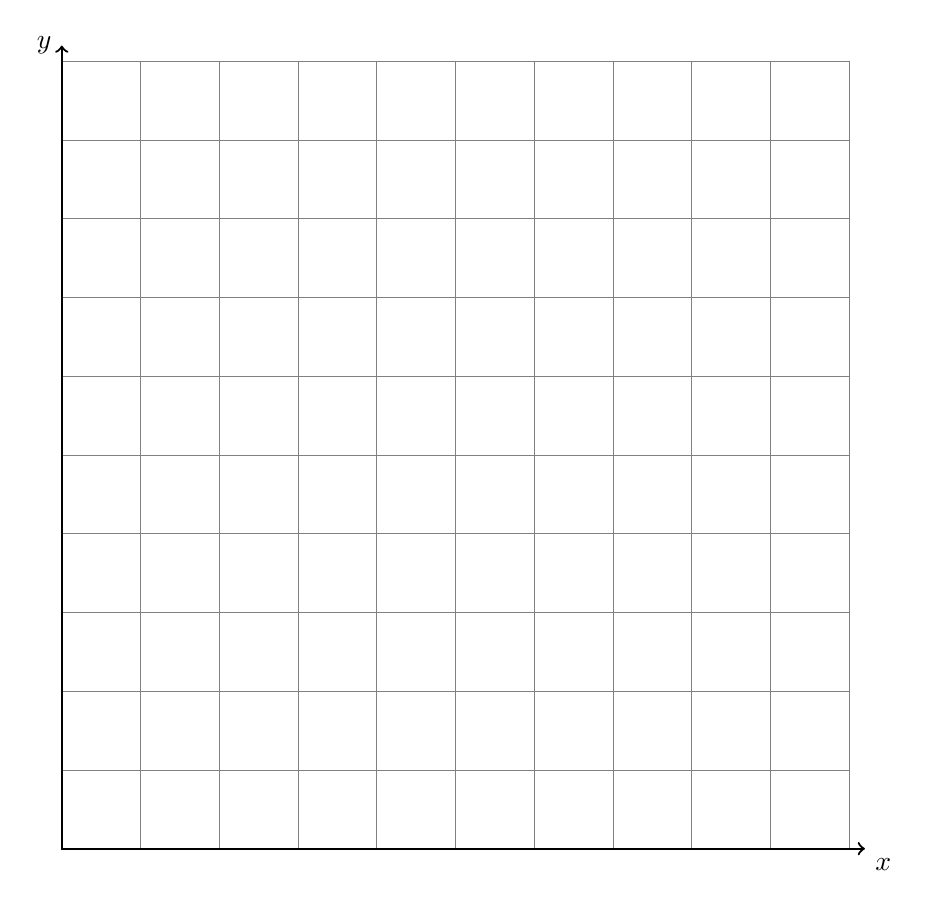
\begin{tikzpicture}%[scale=0.4]
    \draw [help lines] (0,0) grid (10,10);
    \draw [thick, <->] (0,10.2) node [left] {$y$}
         -- (0,0) -- (10.2,0) node [below right] {$x$};
    %\draw[fill] (2,2) circle  [radius=0.05]
         %node[below left] (2, 2) {$A$};
  \end{tikzpicture}

\end{enumerate}
\end{document}
